% !TEX encoding = UTF-8 Unicode

\documentclass[a4paper]{article}

\usepackage{color}
\usepackage{url}
\usepackage[utf8]{inputenc} % make weird characters work
\usepackage{graphicx}
\usepackage{amsfonts}
\usepackage{multirow}

\usepackage{amsmath}

\usepackage[english,serbian]{babel}

\usepackage[unicode]{hyperref}
\hypersetup{colorlinks,citecolor=green,filecolor=green,linkcolor=blue,urlcolor=blue}


\begin{document}

\title{Vrste beskonačnosti. Paradoks Hilbertovog hotela\\ \small{Seminarski rad u okviru kursa\\Tehničko i naučno pisanje\\ Matematički fakultet}}

\author{Milica Zubljić\\ \small{mi22047@alas.matf.bg.ac.rs}\\ Branko Katanić\\ \small{mi22219@alas.matf.bg.ac.rs}\\ Dimitrije Spasojević\\ \small{mi22042@alas.matf.bg.ac.rs}\\ Luka Tonić\\ \small{mi22102@alas.matf.bg.ac.rs}}
\date{14.~novembar 2022}
\maketitle

\abstract{
U ovom seminarskom radu bavimo se problemom prebrojivosti. Pitamo se: da li je moguće smestiti „beskonačno” gostiju u nekakav „beskonačni” hotel? Da bismo znali kako bi uopšte to bilo moguće, pozabavili smo se samim pojmovima beskonačnosti i prebrojivosti. Uspeli smo da nađemo rešenje za deo problema. Deo problema ostao je nerešen, ali u nastavku dajemo dobro objašnjenje zašto je tako. \\%U ovom seminarskom radu biće govora o pojmu beskonačnosti. Objasnićemo šta je to beskonačnost, da li postoji više vrsta beskonačnosti, kako se interpretira beskonačnost u svakodnevnom životu itd. Ovaj interesantan koncept, kao i njegova (ne)pojmljivost ljudskom umu, biće ilustrovani kroz primer čuvenog paradoksa Hilbertovog beskonačnog hotela.\\

ključne reči: beskonačnost, prebrojivost, neprebrojivost
}

\newpage

\tableofcontents %sadržaj

\newpage

\section{Uvod}
\label{poglavlje:uvod}

Svima nama dobro je poznat koncept beskonačnosti. U svakodnevnom razgovoru, ma o kojoj temi se razgovaralo, ovaj pojam se neretko javlja i ne iziskuje nikakvo objašnjavanje. No, da li možemo sa sigurnošću tvrditi da umemo da pojmimo taj opštepoznati koncept? Da li je pojam beskonačnosti jednoznačan ili, pak, ima potrebe precizirati njegovo značenje? Odgovore na ova pitanja naći ćete u nastavku teksta. Ovaj interesantan koncept, kao i njegova (ne)pojmljivost ljudskom umu, biće ilustrovani
kroz primer čuvenog paradoksa Hilbertovog beskonačnog hotela.\\

Prva istraživanja pojma beskonačnosti otpočela su još vekovima pre nove ere. Ovim pojmom bavili su se žitelji Starog Egipta i Stare Grčke, kolevke moderne kulture. Jedan od prvih ljudi zainteresovanih za taj pojam bio je čuveni antički filozof Zenon iz Eleje\footnote{Zenon (Eleja, 490-430. g.p.n.e.) - grčki filozof, pripadnik elejske škole koju je osnovao Parmenid}. U filozofiji, beskonačno je ono što je neograničeno, što ide izvan bilo koje utvrđene granice\cite{weyl2013levels}.\\

Kada biste pitali decu koji je najveći broj koji postoji, verovatno bi vam rekla: beskonačno. Ako posmatramo problem na taj način, mogli biste im odvratiti da je broj veći od beskonačno: beskonačno plus jedan. Tako možemo ići u nedogled, ali poenta je da u matematici beskonačno \textbf{nije brojevna vrednost}. Ona zapravo označava nešto što nije konačno, nešto veoma veliko. Ako uzmemo za primer neku promenljivu, ona ne može biti jednaka beskonačnosti, ali može joj težiti. U tom kontekstu, pojam beskonačnosti koristi se u radu sa limesima, integralima, geometrijskim redovima itd.\\

\section{Zanimljivosti o beskonačnostima}

Simbol beskonačnosti '$\infty$' uveo je britanski matematičar Džon Volis (eng. John Wallis) u 17. veku. Taj simbol nastao je po uzoru na stari zapis rimskog broja hiljadu, koji je takođe označavao neki veoma veliki broj. (slika \ref{fig:Uzor za simbol beskonačnosti danas})\cite{beskonačno2016}
    
\begin{figure}[ht!]
\begin{center}

\includegraphics[scale=0.75]{Simbol.PNG}
\end{center}
\caption{Uzor za simbol beskonačnosti danas}
\label{fig:Uzor za simbol beskonačnosti danas}
\end{figure}
    
U alhemiji, grani filozofije prirode iz koje su se razvile moderne nauke kao što su hemija i farmakologija, beskonačnost je predstavljao Uroboros, zmaj sa repom u ustima koji neprestano proždire samog sebe. (slika \ref{fig:Uroboros})
    
\begin{figure}[ht!]
\begin{center}
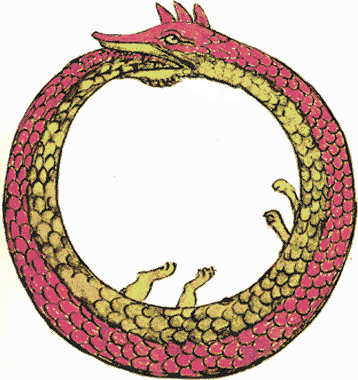
\includegraphics[scale=0.4]{Uroboros.png}
\end{center}
\caption{Uroboros}
\label{fig:Uroboros}
\end{figure}

\newpage

\section{Kardinalnost skupa. Pojam prebrojivosti}
\label{poglavlje:Kardinalnost. Pojam prebrojivosti}

Znamo da postoje brojevni skupovi koji nemaju konačan broj elemenata. Takvi su osnovni skupovi kojima rukujemo u matematici: prirodni, celi, racionalni, iracionalni i realni brojevi.

Nama najintuitivniji od njih jeste skup prirodnih brojeva ($\mathbb{N}$). U teoriji, možemo početi da brojimo od 1 pa nadalje (2,3,4,...) i da budemo sigurni da nijedan broj nismo preskočili u procesu, iako taj proces nema kraja. Tako bismo naveli sve prirodne brojeve (za beskonačno dug vremenski period). Slično tome, možemo brojati od 0 naniže i pokriti skup celih brojeva ($\mathbb{Z}$). Kod skupa racionalnih brojeva ($\mathbb{Q}$) malo je kompleksniji postupak\footnote{Tabela čije su prva vrsta ($p$) i prva kolona ($q$) prirodni brojevi (1,2,3,...). U presecima odgovarajućih vrsta i kolona dobijaju se racionalni brojevi oblika $\frac{p}{q}$, a nabrajaju se po dijagonalama ($\frac{1}{1}, \frac{2}{1}$, $\frac{1}{2}$, $\frac{1}{3}$, $\frac{2}{2}$, $\frac{3}{1}$,...)
}, ali njegovom primenom takođe možemo biti sigurni da nijedan broj nismo ispustili.

Pošto članove navedenih skupova možemo poređati u niz iako ih ima beskonačno mnogo, kažemo da oni imaju \textbf{prebrojivo mnogo} elemenata. Formalnije, za neki skup kažemo da je prebrojiv ako postoji bijekcija $f$ sa skupa prirodnih brojeva u taj skup\cite{klaric2016}.

Dakle, govorimo o \textbf{prebrojivoj beskonačnosti}. Ona se u matematici obeležava sa $\aleph_{0}$ ($\aleph$ - prvo slovo hebrejske azbuke).\\

S druge strane, govoreći o skupovima iracionalnih ($\mathbb{I}$) i realnih ($\mathbb{R}$) brojeva, ne postoji metoda kojom bismo njihove elemente mogli poređati u niz i sve ih pobrojati. Zato kažemo da ovakvi skupovi imaju \textbf{neprebrojivo mnogo} elemenata i govorimo o \textbf{neprebrojivoj beskonačnosti}. Više o tome u poglavlju \ref{poglavlje:Princip neprebrojivosti}.


\newpage

\section{Pojam prebrojive beskonačnosti}
\label{poglavlje:Pojam prebrojive beskonačnosti}
U 19. veku Georg Kantor uveo je pojam kardinalnosti i prebrojivosti skupova. Njegova teorija naišla je na osudu tadašnjih cenjenih matematičara.
Jedan od ljudi koji je ipak prepoznao njen značaj bio je David Hilbert\footnote{David Hilbert (Kenigsberg, 1862-1943) - nemački matematičar}.
On je uspeo da nam vrlo slikovito približi pojam beskonačnosti, opisavši problem smeštanja beskonačno mnogo gostiju u hotel sa beskonačno mnogo soba - \textbf{Hilbertov hotel.}

\subsection{Hilbertov hotel}
Hilbertov hotel je hotel koji ima beskonačno mnogo soba i sve su popunjene. Da li u njega ipak može stati jos gostiju?

\subsubsection{Konačan broj novih gostiju}
\label{potpotpoglavlje:Konačan broj novih gostiju}
Dakle, ispred potpuno punog hotela nalazi se jedan gost koji traži sobu. Kako rešiti ovaj problem?

Novu sobu možemo osloboditi ako zamolimo gosta iz sobe 1 da pređe u sobu 2, gosta iz sobe 2 da pređe u sobu 3 i tako dalje. Dakle, gost iz sobe $n$ prelazi u sobu $n+1$.
Pošto na raspolaganju imamo beskonačan broj soba, za svaku sobu $n$ postojaće soba $n+1$, pa ćemo lako smestiti sve goste u nove sobe i tako osloboditi sobu broj 1.
Ovaj isti postupak može se primeniti na bilo koji konačan broj gostiju. Na primer, ako treba osloboditi 100 novih soba, svakog gosta ćemo premestiti iz njegove sobe u sobu čiji je broj za 100 veći.

Na malo komplikovaniji problem nailazimo kada na red ne čeka konačan broj gostiju.\\

\subsubsection{Beskonačan broj gostiju}
\label{potpotpoglavlje:Beskonačan broj gostiju}
Pred hotelom se sada nalazi beskonačno veliki autobus sa \textbf {prebrojivo} beskonačno mnogo putnika.
U našem primeru Hilbertovog hotela, jasno je da je činjenica da gostiju ima \textbf {prebrojivo} ključna ako hoćemo da ih rasporedimo po sobama.
Ovaj problem možemo rešiti tako što ćemo gosta iz prve sobe zamoliti da pređe u drugu, gosta iz druge u četvrtu, iz treće u šestu i tako dalje.
Uopšteno, gost iz sobe \textbf{n} prelazi u sobu \textbf{2n}. Ovim procesom oslobodili smo sve sobe sa neparnim brojem.
Pošto neparnih brojeva ima beskonačno mnogo, to ostavlja dovoljno mesta za sve putnike beskonačno velikog autobusa.\\

\flushleft{\large{\textbf{Dokaz o beskonačnosti skupa neparnih brojeva}}}
\vspace{0,5cm}

Pretpostavimo suprotno, to jest da je skup neparnih brojeva konačan.
To znači da postoji najveći broj $n$ iz tog skupa.
Svaki neparni broj možemo zapisati u obliku $2p+1$, gde je $p$ bilo koji ceo broj, pa tako možemo zapisati i ovaj najveći broj.
Sada razmatrajmo broj $n+2$: $n+2=2p+1+2=2(p+1)+1$.
Broj $2(p+1)$ očigledno je paran, pa zaključujemo da je broj $n+2$ neparan, a u isto vreme veći od najvećeg neparnog broja.
Ovim zaključkom dolazimo do kontradikcije, što znači da smo dokazali da neparnih brojeva ima beskonačno mnogo.



\newpage

\subsubsection{Beskonačan broj autobusa sa po beskonačno mnogo gostiju}
\label{potpotpoglavlje:Beskonačan broj autobusa sa po beskonačno mnogo gostiju}
Ovog puta imamo beskonačnu kolonu beskonačno velikih autobusa, sa po \textbf {prebrojivo} beskonačno putnika. Da bismo svakom novom gostu dodelili sobu, potrebno je svakom već postojećem gostu dodeliti prvi prost broj, 2, stepenovan brojem njihove sobe. Tako gost iz sobe broj 7 odlazi u sobu broj $2^7$, a to je soba 128. Zatim se gostima iz prvog od beskonačnih autobusa dodeljuje soba broj: sledeći prost broj, 3, stepenovan brojem njihovog sedišta u autobusu. Tako osoba na sedištu broj 7 u prvom autobusu odlazi u sobu broj $3^7$ to jest u sobu 2.187. To se nastavlja za ceo prvi autobus. Putnicima iz drugog autobusa se dodeljuju eksponenti sledećeg prostog broja, 5. Sledećem autobusu, eksponenti broja 7. Sledećim autobusima: eksponenti broja 11, eksponenti broja 13, broja 17 i tako dalje. Pregledan prikaz ovog postupka može se videti u tabeli \ref{tabela:Tabela1}.

\hspace{10cm}
\begin{table}[h!]
\begin{center}
\caption{Dodela soba gostima}
\renewcommand{\arraystretch}{1.5}
\setlength{\tabcolsep}{4pt}
  \begin{tabular}{ |c|c|c|c|c|c|c|c| }
    \hline
    Dodeljivanje&\multicolumn{7}{ |c| }{Broj sobe} \\\cline{2-8}
    sobe&1&2&3&4&5&...&$n$\\\hline
    Trenutni gosti&$2^1$&$2^2$&$2^3$&$2^4$&$2^5$&...&$2^n$\\\hline
    Autobus 1&$3^1$&$3^2$&$3^3$&$3^4$&$3^5$&...&$3^n$\\\hline
    Autobus 2&$5^1$&$5^2$&$5^3$&$5^4$&$5^5$&...&$5^n$\\\hline
    Autobus 3&$7^1$&$7^2$&$7^3$&$7^4$&$7^5$&...&$7^n$\\\hline
    Autobus 4&$11^1$&$11^2$&$11^3$&$11^4$&$11^5$&...&$11^n$\\\hline
    ...&...&...&...&...&...&...&...\\\hline
    Autobus $n$&${P_{n+1}}^1$&${P_{n+1}}^2$&${P_{n+1}}^3$&${P_{n+1}}^4$&${P_{n+1}}^5$&...&${P_{n+1}}^n$\\\hline
  \end{tabular}
  \label{tabela:Tabela1}
\end{center}
\end{table}

\hspace{7cm}

\flushleft{\large{\textbf{Euklidov dokaz: beskonačno prostih brojeva}}}
\vspace{0,5cm}

Euklid je izneo dokaz da prostih brojeva ima beskonačno mnogo u svom delu „Elementi”\cite{williamson1788elements}.

Neka je dat bilo koji konačni skup prostih brojeva $p_{1}, p_{2}, ..., p_{n}$. Biće pokazano da postoji barem još jedan prost broj koji se ne nalazi u tom skupu.

Neka je $P$ proizvod svih prostih brojeva u skupu: $P = p_{1}p_{2}...p_{n}$. Neka je $q = P + 1$. Tada $q$ ili jeste ili nije prost broj:
\begin{itemize}
\item Ako je $q$ prost, onda postoji bar jedan broj ($q$) koji je prost, a nije u prvobitnom skupu.
\item Ako $q$ nije prost, onda neki prost broj $p$ deli $q$. Kad bi ovaj broj $p$ bio u skupu, tada bi on delio $P$ (jer je $P$ proizvod svih brojeva u skupu); ali $p$ deli $P + 1 = q$. Ako $p$ deli $P$ i $q$, onda bi $p$ morao da deli razliku\footnote{U opštem slučaju, za svaka tri cela broja a, b, c važi: ako $a \mid b$ i $a \mid c$ onda $a \mid (b - c)$} ova dva broja, što je $(P + 1) - P$ ili jednostavno 1. Kako nijedan prost broj ne deli 1, $p$ ne može biti u skupu. Ovo znači da barem još jedan prost broj mora postojati mimo onih koji su već u skupu.
\end{itemize} 

Ovo dokazuje da za svaki konačni skup prostih brojeva postoji prost broj koji nije u tom skupu i stoga prostih brojeva mora biti beskonačno mnogo.

\section{Princip neprebrojivosti}
\label{poglavlje:Princip neprebrojivosti}

\newline

Do sada smo imali primere smeštanja i konačnog i beskonačnog broja osoba u Hilbertov hotel. Primetimo da su u svim dosadašnjim primerima gosti koje je trebalo smestiti u Hilbertov hotel bili na neki način numerisani (brojem sedišta i brojem autobusa). To nam je pomoglo da formiramo preslikavanje koje obezbeđuje da se svi gosti smeste, ali šta ako gosti koji dolaze ne mogu biti numerisani prirodnim brojevima? Šta ako dolazi tura gostiju kojih ima onoliko koliko ima tačaka na brojevnoj pravoj? 
\newline
Kao odgovor na postavljena pitanja potrebno je uvesti pojam neprebrojivosti. Za skup koji nije prebrojiv, ili za koji je nemoguće pronaći bijektivnu funkciju koja preslikava skup prirodnih brojeva u dati skup, kaže se da je neprebrojiv. 
\subsection{Dokaz o neprebrojivosti skupa realnih brojeva}

Da bismo dokazali da je skup realnih brojeva neprebojiv, problem ćemo prvo svesti na manji skup. 
Prvo ćemo dokazati da je skup x$\in$(0,1) neprebrojiv.
\newline
Pretpostavimo suprotno, to jest da je skup x$\in$(0,1) prebrojiv \cite{matematicka_logika}. Prvo moramo da primetimo da proizvoljan broj iz intervala (0,1) nema jedinstveni zapis ($1/4=0.2500000$ i $1/4=0.249999$). Dogovorićemo se da koristimo oblik broja koji sadrži konačan broj nenula decimala ($1/4=0.249999$) bez gubljenja na opštosti. Pretpostavkom da je skup x$\in$(0,1) prebrojiv, zaključujemo da se taj skup može zapisati u obliku niza: $$\{x_{1},x_{2},x_{3},...,x_{n}\}$$.
\newline
Brojeve datog niza u tom slučaju možemo predstaviti na sledeći način:

\begin{align*}
    x_{1} & = 0,\color{red}a_{11}\color{black}a_{12}a_{13} \ldots a_{1n} \ldots \\
    x_{2} & = 0,a_{21}\color{red}a_{22}\color{black}a_{23} \ldots a_{2n} \ldots \\
    x_{3} & = 0,a_{31}a_{32}\color{red}a_{33}\color{black} \ldots a_{3n} \ldots \\
    & \vdots \\
    x_{n} & = 0,a_{n1}a_{n2}a_{n3} \ldots \color{red} a_{nn} \color{black} \ldots \\
    & \vdots 
\end{align*}

\newline
Posmatrajmo niz brojeva koji dobijamo na dijagonali date šeme:

$$a_{11},a_{22},a_{33} \ldots a_{nn}$$\\

\par 
Formirajmo decimalni broj gde je:
$$
a_{k} = \left\{\begin{array}{lr}
        5, & \text{ako je } a_{kk} = 5\\
        1, & \text{ako je } a_{kk} \not= 5\\
        \end{array} 
$$
\newline
Takav broj nismo dobili u šemi, a s obzirom na to da smo počeli sa pretpostavkom da $x\in(0,1)$ i da smo sve brojeve prikazali u šemi, dolazimo do kontradikcije. Skup brojeva u intervalu (0,1) je neprebrojiv, što dalje dovodi do zaključka da je skup realnih brojeva takođe neprebrojiv.\\

\newline
Pošto važi $\mathbb{Q}\subset \mathbb{R}$, zaključujemo da je neprebrojiva beskonačnost brojnija od prebrojive. Ona se obeležava sa $c$, a ne sa $\aleph_{1}$, na šta se može naići u literaturi. Razlog takvog označavanja je činjenica da ne znamo da li postoji beskonačnost koja je „veća” od prebrojive, a „manja” od neprebrojive, tj. ne znamo je li $c$ prvi sledbenik $\aleph_{0}$.\\
\subsection{Hilbertov hotel i neprebrojivo mnogo gostiju}
Hilbertov hotel ima beskonačno mnogo numerisanih soba, samim tim zaključujemo da ima prebrojivo mnogo beskonačno soba. Ukoliko pokušamo da smestimo neprebrojivo mnogo gostiju u hotel sa prebrojivo mnogo soba, nećemo uspeti jer znamo da neprebrojiv skup ima više elemenata nego prebrojiv skup.

\section{Zaključak}
\label{poglavlje:Zaključak}
Pojam kardinalnosti skupa postaje neintuitivan kada se izađe izvan opsega konačnosti. Paradoks Hilbertovog hotela služi kao dobar primer pomoću kojeg je nakon upotrebe matematičkih aparata moguće uvideti primenu, značaj i značenje apstraktnih koncepata kao što je beskonačnost. Svakodnevno se susrećemo sa različitim skupovima brojeva poput skupa prirodnih, racionalnih ili realnih brojeva, ali njihove osobine, a samim tim i prirodu je između ostalog najbolje moguće razumeti tek nakon analize njihove kardinalnosti, što je i glavni motiv za detaljnu analizu različite vrste beskonačnosti i za analizu paradoksa Hilbertovog hotela.

\newpage

\addcontentsline{toc}{section}{Literatura}

\renewcommand{\refname}{Literatura}
\bibliographystyle{apalike}
\bibliography{Literatura}

\end{document}
